\documentclass{report}
\usepackage[utf8]{inputenc}
\usepackage{graphicx}
\usepackage[portuguese]{babel}
\usepackage[margin=2cm]{geometry}

\title{ 
\includegraphics[scale=0.3]{logo.png} \\ \textbf{Off Constructions - O uso de bases de dados aplicadas à construção civil}}

\author{Bases de Dados \\ Mestrado Integrado em Engenharia Informática e Computação \\ \\ G504 \\ Afonso Carvalho up201807481@fe.up.pt \\ Tiago Rodrigues up201907021@fe.up.pt \\ Tomás Fidalgo up201906743@fe.up.pt}

\graphicspath{{./images/}}

\begin{document}
	\maketitle
	
	\tableofcontents
	
	\chapter{Introdução}
		\paragraph{}A OFF Constructions, uma empresa de construção sediada no Porto, pretende
		armazenar informação relativa ao seu funcionamento, com o propósito de tornar o seu
		negócio mais eficiente. Deste modo, foi-lhes sugerida a seguinte base de dados:
		
		\section{Requisitos do cliente}
		
			\paragraph{•}Do cliente é guardada informação relativa à sua identificação, por
			motivos de faturação. Assim, é necessário guardar o nome, o contacto telefónico, a
			morada e o seu NIF. Quando o cliente requisita uma obra, é primeiro criado um
			projeto, que contém detalhes relativos ao orçamento acordado e ao prazo de
			finalização. Um cliente pode requisitar mais do que uma obra, no entanto, cada
			obra terá apenas um cliente, seja ele particular ou outra empresa.
		
		\section{Requisitos da obra}
		
			\paragraph{•}De cada obra interessa saber a sua localização (rua, nº de porta,
			código postal e cidade), a data de início das construções, o custo real (que tanto
			pode ser superior como inferior ao orçamento), a área de terreno envolvida assim
			como a área interior projetada. Por fim, é necessário saber, a um dado instante, o
			estado da obra.
			
		\section{Requisitos de material}
			
			\paragraph{•}Cada obra tem, de antemão, uma certa quantidade de material
			alocado, do qual se pretende saber a quantidade disponível e o custo. Cada
			material diferente possui um código interno, assim como uma designação pela qual
			é conhecido. Este material é guardado num dos estaleiros da empresa (a OFF
			Constructions prefere guardar todo o material igual no mesmo estaleiro), dos
			quais é importante saber a localização (com os mesmos requisitos da obra) e
			capacidade máxima.
			
		\section{Requisitos de veículos}
		
			\paragraph{•}Para além do material, a empresa possui uma frota de veículos,
			tanto de transporte de empregados como de materiais, assim como todos os tipos
			de maquinaria pesada usada nas diferentes obras. De cada veículo, a empresa
			gostaria de registar a matrícula, a categoria (segundo o código da estrada), as
			despesas associadas, o consumo médio do veículo bem como a data de inspeção de
			cada um.
			
		\section{Requisitos dos empregados}
		
			\paragraph{•}Por último, a OFF gostaria de registar todos os seus empregados no
			sistema. Todos os empregados têm o seu nome, NIF, contacto e salário registados,
			assim como a sua habilitação escolar. Dos empregados que estão nas obras,
			interessa saber a sua especialidade (carpinteiro, eletricista, etc.) e o cargo
			que possui na obra. Quanto aos empregados que estão no escritório, é necessário
			guardar a sua estação de trabalho e a sua especialização (decorador,
			contabilista, arquiteto, engenheiro, entre outras). Outro tipo de empregados que
			a OFF contrata são maquinistas, cujo trabalho é operar e manobrar os vários
			veículos usados nas obras. Posto isto, de cada um deles é necessário saber as
			categorias (segundo o código da estrada) que estão habilitados a conduzir.
				
			\begin{figure}[hb!]
				\centering
				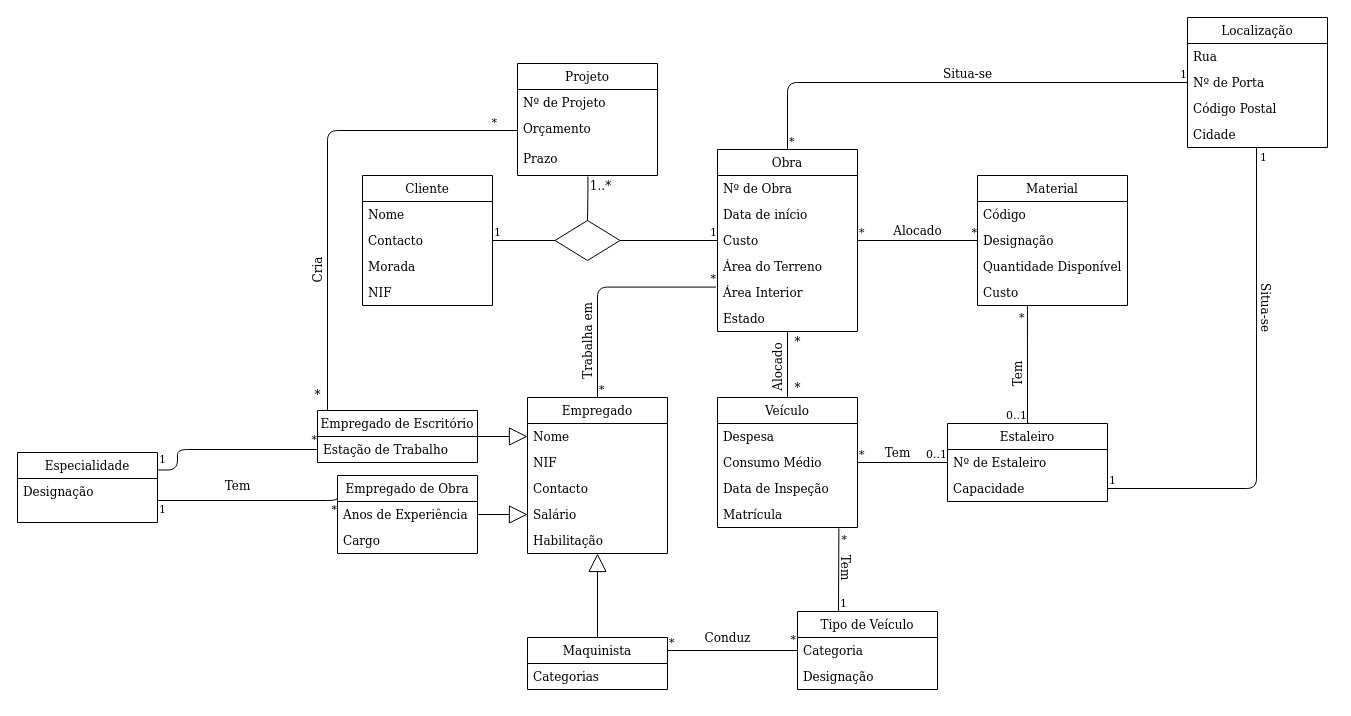
\includegraphics[scale=0.45, angle=-90]{UML-Original.png}
				\caption{Diagrama UML original correspondente aos requisitos dados}
			\end{figure}
		
		\section{Novos requisitos}
			
			\paragraph{•}Após falar com o docente, foram propostas algumas ligeiras
			alterações ao modelo apresentado, as quais podem ser vistas no seguinte diagrama
			UML.
			
			\begin{figure}[hb!]
				\centering
				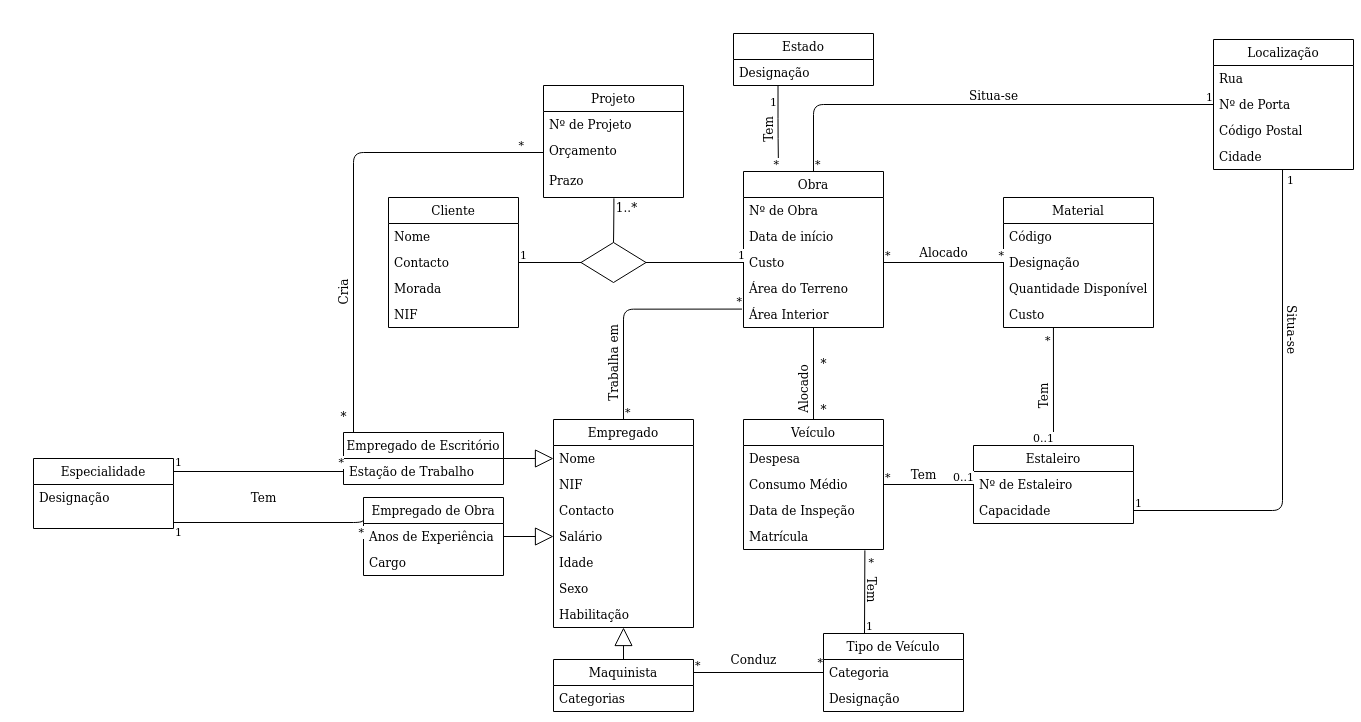
\includegraphics[scale=0.44, angle=-90]{UML-Revisto.png}
				\caption{Diagrama UML revisto correspondente aos novos requisitos}
			\end{figure}
	\chapter{Esquema Relacional}
	
		\paragraph{•}O diagrama UML revisto poderá ser decomposto no seguinte esquema
		relacional, e são possíveis obter as seguintes tabelas.
		
		\begin{itemize}
			\item $Cliente(Nome, Morada, Contacto, NIF)$
			\item $Projeto( N de Projeto, Orcamento, Prazo)$
			\item $Obra(N de Obra, Data de Inicio, Custo, Area do Terreno, Area Interior,
			Estado \rightarrow Estado, Rua \rightarrow Localizacao.Rua,\\ N de Porta
			\rightarrow Localizacao.N de Porta, Codigo Postal \rightarrow
			Localizacao.Codigo Postal)$
			\item $Estado(Designacao)$
			\item $Material(Codigo, Designacao, Quantidade Disponivel, Custo, Guardado
			\rightarrow Estaleiro)$
			\item $Localizacao(Rua, N de Porta, Codigo Postal, Cidade)$
			\item $Estaleiro(N de Estaleiro, Capacidade, Rua \rightarrow Localizacao.Rua, N
			de Porta \rightarrow Localizacao.N de Porta, Codigo Postal \rightarrow
			Localizacao.Codigo Postal)$
			\item $Veiculo(Matricula, Consumo Medio, Data de Inspecao, Despesa, Tipo 
			\rightarrow TipoDeVeiculo, Guardado \rightarrow Estaleiro)$
			\item $TipoDeVeiculo(Categoria, Designacao)$
			\item $Especialidade(Designacao)$
			\item $Empregado(Nome, NIF,  Contacto, Salario, Habilitacao, Idade, Sexo)$
			\item $EmpregadoDeEscritorio(NIF \rightarrow Empregado, Estacao de Trabalho,
			especialidade \rightarrow Especialidade)$
			\item $EmpregadoDeObra(NIF \rightarrow Empregado, Anos de Experiencia,  Cargo,
			especialidade \rightarrow Especialidade)$
			\item $Maquinista(NIF \rightarrow Empregado, Categorias)$
			\item $Cria(NIF \rightarrow EmpregadoDeEscritorio, N de Projeto \rightarrow
			Projeto)$
			\item $MaterialAlocado(Codigo \rightarrow Material, N de Obra \rightarrow Obra)$
			\item $VeiculoAlocado(Matricula \rightarrow Veiculo, N de Obra \rightarrow Obra)
			$
			\item $TrabalhaEm(NIF \rightarrow Empregado, N de Obra \rightarrow Obra)$
			\item $Conduz(NIF \rightarrow Maquinista, Designacao \rightarrow TipoDeVeiculo)$
			\item $ClienteObraProjeto(Cliente \rightarrow Cliente, Obra \rightarrow Obra,
			Projeto  \rightarrow Projeto)$
		\end{itemize}
		
		
		
\end{document}